\section{Adding buildings}
\label{sec:addingbuildings}
As a player you may want to add buildings to the world. In this section we will explain how a player can add buildings and how we have implemented this feature.

\subsection{Controls and feedback}
For now you can position a castle entity by pressing the 'N' button. You can drag the mouse and a slightly transparent castle will appear at the mouse position. When the player hovers over another static entity, whilst the player is positioning a castle, the texture will get a red border. This will notify the player that the building cannot be placed at that current mouse position. If the player has found a spot on the world where it wants to position the building, it can press 'N' again to set the current position as the final position of the building.

\subsection{States}
We are using the state pattern during positioning and placing buildings, because this pattern makes it easy to extend the behaviour of the player or entity, which can be different each state.\\
When a player hits the 'N' button, the key handler will look at the player its current state. If the player is already in the ChoosingBuildingPosition, then the player wants to 
set the current mouse position as the final position of the building, and the player its state will change to PlacingBuilding.\\
If the player is not in the ChoosingBuildingState, the key handler will call the method 
choosing\_building\_position, which belongs to the BuildingManager. The building manager is responsible for creating the building entity, together with the BuildingFactory.
When the entity is created, it will be added to the world so this object will be rendered.
The BuildingManager will also set the positioning\_object variable of the player, so the player can keep track of the building it is positioning from now on. After all this is done, the state of the player will be changed to ChoosingBuildingPosition.
A state machine diagram explaining state transitions can be found in \cref{fig:statediagram-addingbuildings} and a class diagram with relevant methods, associations and variables can be found in \cref{fig:classdiagram-addingbuildings}.

\begin{figure}[!htb]
    \centering
    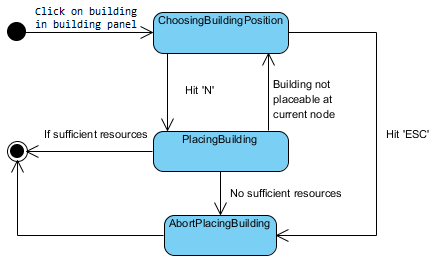
\includegraphics{res/adding-buildings/States-StateDiagram.png}
    \caption{Adding buildings state diagram.}\label{fig:statediagram-addingbuildings}
\end{figure}

\subsubsection{ChoosingBuildingPosition}
At entering this state, the texture its opacity will be set to 70\%. We have chosen to do so, because this will make clear which objects are already placed and which objects are not placed by the player yet.\\
During the execute method of this state the mouse position of the player will be tracked. If the mouse position has changed, the GraphManager will be consumed to get the nearest node in relation to the mouse position. If there is another static entity on that node, we want to inform the player by changing the entity its texture by adding a red border.

\subsubsection{PlacingBuilding}
The PlacingBuilding state will be entered when the player hits 'N' while it is in the ChoosingBuildingPosition state. This state only has logic in its enter method, because it needs to make one decision: can the building be positioned at this position or not.\\
If the building cannot be positioned at the node, the state will be changed back to ChoosingBuildingPosition, to give the user another chance to find a good spot for the building. If the building can be placed at the node, the entity will be added to the building array of the player and to the building array of the BuildingManager. The opacity will also be set to 0\%. The positioning\_object variable kept by the player object will be cleared, just like the current state of the user.

\begin{figure}[!htb]
    \centering
    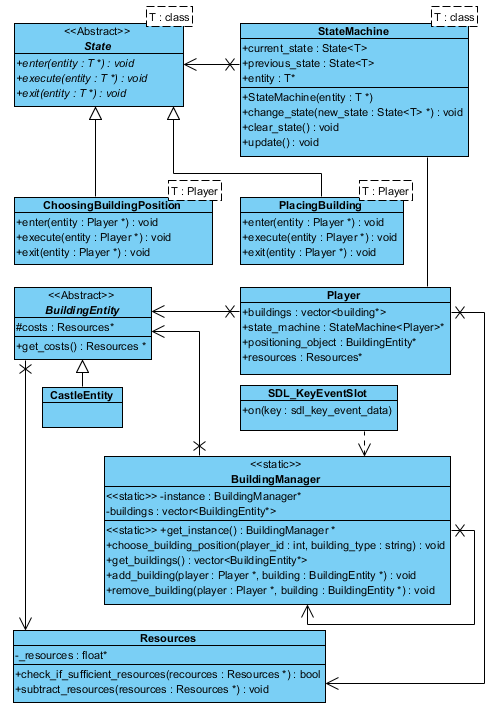
\includegraphics{res/adding-buildings/States-ClassDiagram.png}
    \caption{Adding buildings class diagram.}\label{fig:classdiagram-addingbuildings}
\end{figure}
\clearpage



